
\chapter{Fortgeschrittene Einstellungen}
\label{chap:advanced-settings}

In diesem Kapitel wird drauf eingegangen wie man die viele Einstellungen von Untis an den persönlichen Bedürfnissen angepasst werden können.

\section{Schaltfläche Personalisierung}
\label{sec:advanced-quick-access}

Wird zu einem späteren Zeitpunkt ergänzt.

\begin{wrapfigure}{r}{.05\textwidth}
	\vspace{-45pt}
	
\includegraphics[width=.05\textwidth]{fenstergruppen-symbol}
	\vspace{-35pt}
\end{wrapfigure}

\section{Fenstergruppen}
\label{sec:fenstergruppen}

Fenstergruppen ermöglichen den schnellen Zugriff auf mehrere Fenster, die man oft zusammen einsetzt. Neu in Untis 2015 gibt es die Möglichkeit, Fenstergruppen Ressourcen-spezifisch abzulegen, diese wurde bereits in \secref{sec:standard-fenstergruppen}, bereits erklärt.\\

\begin{wrapfigure}{r}{.4\textwidth}
	\vspace{-14pt}
	\centering
	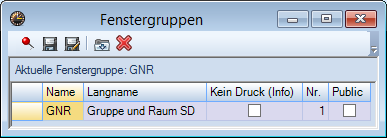
\includegraphics[width=.38\textwidth]{fenstergruppen-ansicht}
	\vspace{-5pt}
	\caption{Fenstergruppen Ansicht}
	\label{fig:fenstergruppen-ansicht}
	\vspace{-14pt}
\end{wrapfigure}

\noindent
Abgesehen von den Ressourcen-spezifischen Standard-Fenstergruppen kann man bis zu 30 Fenstergruppen die über ihre Nummerierung angesprochen werden.\\
\\
Fenstergruppen zu verwalten klickt man auf das Fenstergruppen-Symbol in der obere rechte Ecke. Dies eröffnet das Fenstergruppen-Ansicht.

\subsection{Aktionen}

\begin{wrapfigure}{r}{.05\textwidth}
	\vspace{-14pt}
	
\includegraphics[width=.05\textwidth]{anzeigen-der-fenstergruppe-symbol}
	\vspace{-35pt}
\end{wrapfigure}

\subsubsection{Anzeigen der Fenstergruppe}

\vspace{10pt}

Bringt die markierte Fenstergruppe zum vorschein.\\

\begin{wrapfigure}{r}{.05\textwidth}
	\vspace{-14pt}
	
\includegraphics[width=.05\textwidth]{fenster-nicht-schliessen-symbol}
	\vspace{-35pt}
\end{wrapfigure}

\subsubsection{Fenster nicht schließen}

\vspace{10pt}

Dieses Symbol ändert der Zustand des Fensters in ``nicht-schließbar" \hspace{1pt}. Sämtliche andere Fenstergruppen-Aktionen sind dadurch nicht mehr im Stande die Fenstergruppe-Ansicht selbst zu schließen. Durch ein weitere klick wird er wieder durch die Ausführung manche andere Fenstergruppen-Aktionen geschlossen.\\

\begin{wrapfigure}{r}{.05\textwidth}
	\vspace{-14pt}
	
\includegraphics[width=.05\textwidth]{loschen-symbol}
	\vspace{-35pt}
\end{wrapfigure}

\subsubsection{Löschen}

\vspace{10pt}

\noindent
Die markierte Fenstergruppe wird gelöscht.\\

\begin{wrapfigure}{r}{.05\textwidth}
	\vspace{-14pt}
	
\includegraphics[width=.05\textwidth]{speichern-symbol}
	\vspace{-35pt}
\end{wrapfigure}

\subsubsection{Speichern}

\vspace{10pt}

Speichert die aktuelle Anordnung von Fenstern als eine neue Fenstergruppe. Sollte keine Fenstergruppe markiert sein wird eine ohne Namen angelegt. Bei neue Gruppen empfiehlt es sich eher \texttt{Speichern Unter} zu verwenden.\\

\begin{wrapfigure}{r}{.05\textwidth}
	\vspace{-14pt}
	
\includegraphics[width=.05\textwidth]{speichern-unter-symbol}
	\vspace{-35pt}
\end{wrapfigure}

\subsubsection{Speichern Unter}

\vspace{10pt}

Öffnet ein Dialog, wo man die Name, Langname und Nummer (bis 30) festgelegt werden kann. Danach wird die aktuelle Anordnung von Fenstern als Fenstergruppe gespeichert. Über diese Funktion kann man auch die Namen und Nummerierung von vorhandenen Fenstergruppen anpassen.\\

\subsection{Attribute}

\subsubsection{Kein Druck (Info)}

Die Auswirkungen dieser Attribute sind weder offensichtlich noch Dokumentiert. Bitte daher ignorieren.

\subsubsection{Nr}

\begin{wrapfigure}{r}{.4\textwidth}
	\vspace{-14pt}
	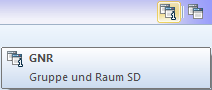
\includegraphics[width=.38\textwidth]{fenstergruppen-mit-tooltip}
	\vspace{-5pt}
	\caption{Fenstergruppen Icon und Tooltip}
	\label{fig:fenstergruppen-mit-tooltip}
	\vspace{-24pt}
\end{wrapfigure}

Da die Icons für Fenstergruppen recht klein sind, haben die Entwickler von Untis sich entschieden die einzelne Fenstergruppen über ihre Nummerierung ersichtlich zu machen. Falls man die Nummerierung nicht merken möchte, werden die Name und Langname in einem Tooltip, sobald man mit der Maus über das entsprechende Icon schwebt, eingeblendet.

\subsubsection{Public}

Fenstergruppen die als \texttt{Public} gekennzeichnet sind, können von allen Benutzer mit entsprechende Rechte angesehen werden.

\section{Formate}
\label{sec:formate}

Wo Fenstergruppen schnellen Zugriff auf mehrere Fenster ermöglichen, ermöglichen Formate den schnellen Zugriff auf Informationen, inden man Fenster seine Informationsverbrauch und sein Umgang mit dem Programm anpasst, z.B. durch eingeblendete Attribute, Font-Anpassungen, etc.\\
\\
Formate erreicht man am leichtesten im Reiter \texttt{Dateieingabe} über \texttt{Formate} im Rubrik \texttt{Werkzeuge}.

\begin{figure}[h]
	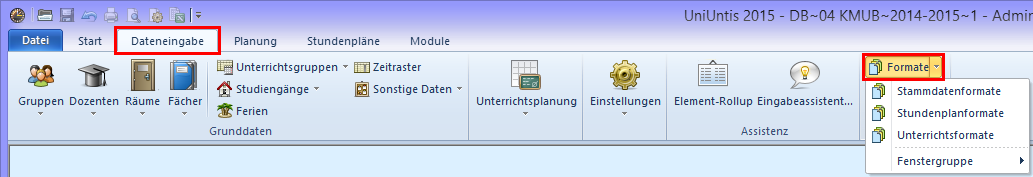
\includegraphics[width=1\textwidth]{formate-menu}
	\vspace{-15pt}
	\caption{Formate: Menüführung}
	\label{fig:formate-menu}
\end{figure}

\newpage

\begin{wrapfigure}{r}{0.4\textwidth}
	\centering
	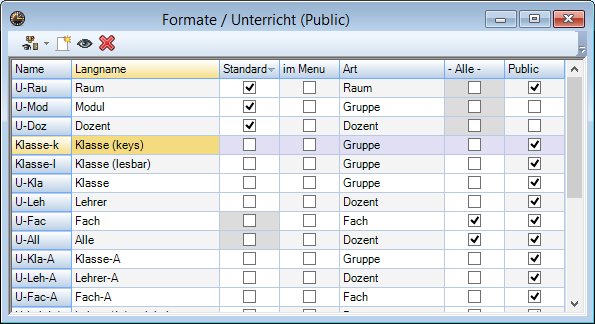
\includegraphics[width=.38\textwidth]{formate-unterricht-schnittstelle}
	\vspace{-5pt}
	\caption{Formate: Unterricht-Ansicht}
	\label{fig:formate-unterricht-schnittstelle}
	\vspace{-15pt}
\end{wrapfigure}

\noindent
Es gibt drei Formatierbare Ansichtstyps: Stammdaten, Unterrichte und Stundenpläne. Unabhängig von diesem Typ haben alle Format-Ansichten die gleiche verfügbare Aktionen, einen Namen und Langnamen, eine Art (Ressourcentyp), sowie spalten zur Einstellung der Anzeige-Ort und Verfügbarkeit. Aus irgendeinem Grunde ist die Art bei Stundenplan-Formate nicht explizit angegeben, dennoch auswählbar.\\

\subsection{Aktionen}

\begin{wrapfigure}{r}{.05\textwidth}
	\vspace{-25pt}
	
\includegraphics[width=.05\textwidth]{ansicht-anzeigen-symbol}
	\vspace{-35pt}
\end{wrapfigure}

\subsubsection{Ansicht Anzeigen}

\vspace{10pt}

\noindent
Eröffnet die markierte Format des Ansichtstyps.\\

\begin{wrapfigure}{r}{.05\textwidth}
	\vspace{-25pt}
	
\includegraphics[width=.05\textwidth]{neu-symbol}
	\vspace{-35pt}
\end{wrapfigure}

\subsubsection{Neu}

\vspace{10pt}

\noindent
Das Klicken des Neu-Symbols bewirkt nur das erzeugen eines neues Formates bei Stundenpläne. Stammdatenformate und Unterrichtsformatte müssen von der jeweilige Ansicht erzeugt werden.\\

\begin{wrapfigure}{r}{.05\textwidth}
	\vspace{-25pt}
	
\includegraphics[width=.05\textwidth]{loschen-symbol}
	\vspace{-35pt}
\end{wrapfigure}

\subsubsection{Löschen}

\vspace{10pt}

\noindent
Hat man ein, von einem Benutzer erstellten, Format markiert wird er beim anklicken des Symbols gelöscht.\\

\begin{wrapfigure}{r}{.06\textwidth}
	\vspace{-25pt}
	
\includegraphics[width=.06\textwidth]{ressource-auswahl-symbol}
	\vspace{-35pt}
\end{wrapfigure}

\subsubsection{Ressourcenauswahl}

\vspace{10pt}

\noindent
Schränkt die angezeigten Ansichtsformate auf die der ausgewählte Ressource ein. Die Ressourcen die zur Auswahl stehen sind abhängig von der Art des Formats: Stammdaten, Unterrichte oder Stundenpläne.\\ 

\subsection{Attribute}

\subsubsection{Standard}
Man soll hiermit entscheiden können ob diese als Standard-Format einsetzen soll. Leider funktioniert dies nicht, denn vieles an Klärungsbedarf würde hiermit entfallen. (Ignorieren)

\subsubsection{im Menu}
Mit dieser Angabe kann man entscheiden ob das Format im jeweiligen Ressourcenmenü erscheinen soll. Diese funktioniert und erleichtert die Benutzung des Programms sehr. (Empfohlen)

\subsubsection{- Alle -}
Diese Angabe scheint wirkungslos zu sein und ist nur bei Format-Typ Unterricht vertreten. Sie wird weder im Untis eigene Dokumentation vorgeführt, noch gibt es einen Tooltip. (Ignorieren)

\subsubsection{Public}
Diese Angabe macht die Ansicht für andere Benutzer sichtbar und kann ich nur empfehlen, wenn mehrere Kollegen die gleiche sicht auf Daten und/oder Pläne haben sollten. Im Zusammenspiel mit der Angabe \texttt{im Menu}, werden entsprechend andere Benutzer auch dieses Format im Stammdatenmenü verwenden können. (Empfohlen)

\section{Stundenplan-Einstellungen}
\label{sec:stundenplan-einstellungen}

\begin{wrapfigure}{r}{0.4\textwidth}
	\vspace{-14pt}
	\centering
	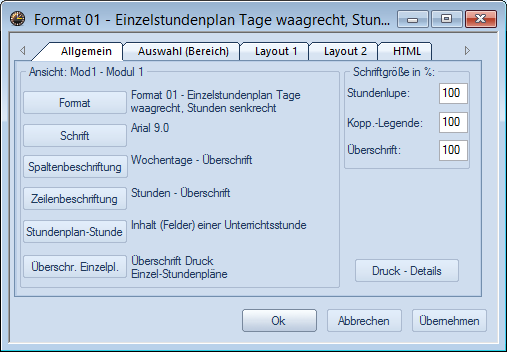
\includegraphics[width=.38\textwidth]{stundenplan-einstellungen}
	\vspace{-5pt}
	\caption{Stundenplan Einstellungen}
	\label{fig:stundenplan-einstellungen}
	\vspace{-50pt}
\end{wrapfigure}

Alle Stundenplan-Ansichten haben die gleiche Einstellung-Ansicht, wie im \figref{fig:stundenplan-einstellungen}. In der Stundenplan-Einstellungen ist der Reiter \texttt{Allgemein} immer als erstes geöffnet. Hier werden weitere untergeordnete Ansichten sowohl über Knöpfe als auch über weitere Reiter verlinkt. Diese Ansichten werden hier gleicht gehandhabt, als die Zuordnung zu einem Kopf oder Reiter ziemlich willkürlich gehandhabt wurde.\\

\vspace{20pt}

\subsection{Format}

\noindent
Im \texttt{Stundenplanformate} kann man zwischen sechs unterschiedliche Stundenplanformate auswählen. Diese werden wiederum untergeordnet in \texttt{Einzelstundenpläne}, Pläne für eine Ressource, und \texttt{Stundenplan-Übersichtspläne}, in dem mehrere Ressourcen dargestellt werden. Wenn man eine bereits vorhandene Einzelstundenplan- oder Übersichtsplan-Format anpasst, kann man nur andere Formate des gleichen untergeordneten Format auswählen. Bei neu erstellte, wie in \secref{sec:formate} beschrieben, kann man frei zwischen beide Unterformate entscheiden.\\

\newpage

\begin{wrapfigure}{r}{0.4\textwidth}
	\vspace{-14pt}
	\centering
	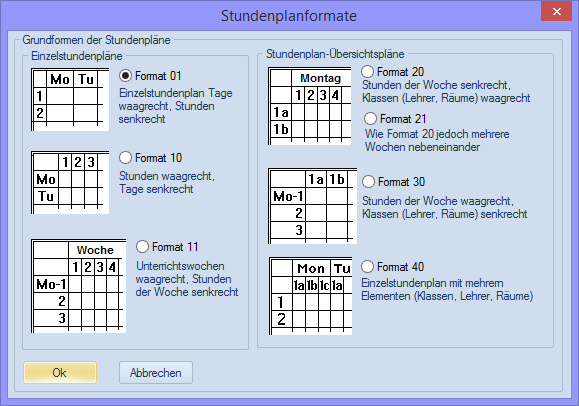
\includegraphics[width=.38\textwidth]{stundenplanformate}
	\vspace{-5pt}
	\caption{Stundenplanformate}
	\label{fig:stundenplanformate}
\end{wrapfigure}

\noindent
\texttt{Format 01}: Ein Einzelstundenplan-Format, in dem Tage die Spalten bilden und Stunden die Zeilen.\\

\noindent
\texttt{Format 10}: Ein Einzelstundenplan-Format, in dem Stunden die Spalten bilden und Tage die Zeilen.\\

\noindent
\texttt{Format 11}: Ein Einzelstundenplan-Format, in dem Schulwochen die Spalten bilden und Wochenstunden die Zeilen.\\

\noindent
\texttt{Format 20}: Ein Übersichtsplan-Format, in dem Wochenstunden die Spalten bilden und Ressource die Zeilen.\\

\noindent
\texttt{Format 21}: Ein Übersichtsplan-Format, in dem Wochenstunden die Spalten bilden und Ressource die Zeilen. Im Gegensatz zu \texttt{Format 20} werden mehrere Wochen hintereinander dargestellt.\\

\noindent
\texttt{Format 30}: Ein Übersichtsplan-Format, in dem Ressourcen die Spalten bilden und Wochenstunden die Zeilen.\\

\noindent
\texttt{Format 40}: Ein Übersichtsplan-Format, in dem Tage und mehrere Ressourcen die Spalten bilden und Stunden die Zeilen. Da man nur eine der Ressourcen kann und die zweite Ressource einfach der nächste aus der List zu sein scheint, ist die Anwendbarkeit dieses Formats stark eingeschränkt.\\

\subsection{Schrift}
\label{sec:schrift}

Hier kann man verschiedene Schrift-Einstellungen machen, wie Schriftart, -stil und -größe. Die Schriftart, die hier ausgewählt wird, wird für alle Elemente des Stundenplans eingesetzt.\\
\\
Der Schriftstil dient als Basis für die anderen Elemente, d.h. die Stil wird für alle Elemente des Plans verwendet, jedoch kann in den anderen Elementen teilweise angepasst werden. Sollte man z.B. ``Fett" \hspace{1pt} auswählen werden alle Elemente in diesem Stil angezeigt. Unterelemente können weiter Stils hinzufügen wie ``Kursiv" \hspace{1pt} oder ``Unterstreichen", aber der Basisstil kann nicht in andere Elemente entfernt werden.\\
\\
Die Größe hier dient auch als Basis auf eine andere Art. Alle Unterelemente des Plans kann man eine prozentuale Große angegeben. Diese wird berechnet nach die hier angegebene Größe. Sollte man hier z.B. 12 auswählen und in einem Element 80\% einstellen wird er etwas kleinder als 12 dargestellt, entsprechend wird 200\% doppelt so groß sein.

\subsection{Spaltenbeschriftung \& Zeilenbeschriftung}

Hier kann man viele unterschiedliche Darstellungsmöglichkeiten für die Spalten- und Zeilenbeschriftung einstellen. Nicht nur Größe und Stil wie in \secref{sec:schrift}, beschrieben, sondern auch die maximale Anzahl der zu darstellenden Zeichen, oder die Bündigkeit bei Zeilen.\\
\\
Darüber hinaus herrscht eine große Vielfalt an Darstellungsmöglichkeiten in Abhängigkeit der zu darstellende Informationen. Eine Stunde kann z.B. durch die Stundennummer, Startzeit oder Start- und Endzeit. Hier kommt das kleine Vorschau-Fenster sehr gelegen und macht weitere Erklärungen gewissermaßen überflüssig.

\subsection{Stundenplan-Stunde}
\label{sec:stundenplan-stunde}

Der Stundenplan-Stunde ist die komplizierteste und gleichzeitig eines der wichtigsten Ansichten, die Untis zu bieten hat. In einer Stundenplan-Stunde kann man, abhängig von der Darstellungsgröße der Stunde, beliebig viele Informationen anzeigen lassen. Dieser Vielfalt ist nicht immer zweckgemäß, bei Übersichtspläne z.B. kann man die gleiche Informationsgehalt, wie in einer Einzelplan, einbauen, dadurch wird sie aber enorm und ziemlich zweckentfremdet da diese meist rein für die Belegungen von Ressourcen verwendet werden.\\
\\
Da Fachbereich KMUB Untis zur Darstellung der Stundenpläne verwendet und recht viel Mühe in dieser gesteckt hat werde ich sie als Beispiel nehmen für was aus ein solcher Stunde rauszuholen ist und welche Probleme dabei entstanden sind. Die Stundenplan-Stunde-Ansicht sowie die in Fachbereich KMUB verwendete Einstellungen können Sie in \figref{fig:stundenplan-stunde} anschauen.

\subsubsection{Fensterbereiche}

\noindent
Ressource (\texttt{Art des Stundenplans}): Ändert die Ressource, die im Plan dargestellt wird. Ein recht gefährlicher Feld, denn sobald geändert gehen fast alle vorhandene Einstellungen verloren. \textbf{Bitte mit bedacht verwenden.}\\

\noindent
Feldchrift Einstellungen (\texttt{Feldart \& Stilknöpfe}): Dieser Bereich passt sich an welches Element selektiert wurde und wird ggf. ergänzt mit der zu Anzeigende Attribut des Elements, wie Kurzname (\texttt{Name}) oder \texttt{Langname}. Diese kann ein wenig verwirrend sein denn die Angaben die hier gemacht werden sind nicht allgemein gültig für die jeweilige Ressource \& Attribute, sondern nur für das Feld. In unserem Beispiel hat Fachbereich KMUB alle drei Fach-Felder eine maximale Anzahl von 45 Zeichen gegeben. Entsprechend werden die Stellen, um die Vorschau möglichst aussagekräftig zu machen, mit dem Zeichen ``x" \hspace{1pt} ergänzt.\\

\noindent
Standardformat (\texttt{Standardstunde}): Ein selten brauchbarer Bereich in dem man sich für das ``Standardformat" \hspace{1pt} entscheiden kann. Auch hier werden viele Einstellungen verworfen sobald das Häkchen gesetzt ist. Auch wenn man nach das Häkchen-setzten \texttt{Abbrechen} drückt wird er gespeichert. Man muss sie bewusst entfernen umn das Standardformat zu umgehen. Wenn das Standardformat verwendet wird, kann man danach lediglich entscheiden ob und welche drei der vier Hauptressourcen in dieser Stunde angezeigt werden sollte. (Die Ressource die in \texttt{Art des Stundenplans} selektiert ist, wird automatisch ausgeschlossen.) Man bekommt nicht mal eine Vorschau denn sowohl im Feinjustierungsbereich als auch im Vorschaubereich erscheint lediglich das Wort ``Standard". \textbf{Bitte mit bedacht verwenden.}\\

\noindent
Feinjustierungsbereich: Hier kann man sowohl einzelne Felder platzieren und deren Größe anpassen als auch die Größe der Stundenplan-Stunde an sich.\\

\noindent
Vorschaubereich: Hier kann man die vorgenommene Einstellungen in ihre Darstellungsgröße anschauen.\\

\begin{figure}[h]
	\centering
	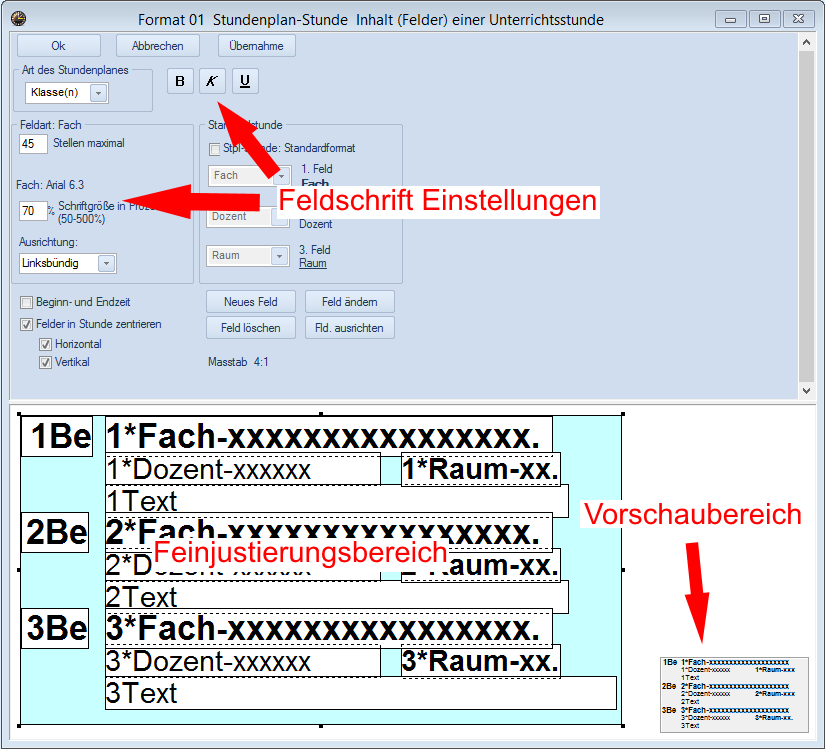
\includegraphics[width=.8\textwidth]{stundenplan-stunde}
	\vspace{-5pt}
	\caption{Stundenplan-Stunde}
	\label{fig:stundenplan-stunde}
\end{figure}

\newpage

\subsubsection{Neues Feld / Feld Ändern}

\begin{wrapfigure}{r}{0.4\textwidth}
	\vspace{-14pt}
	\centering
	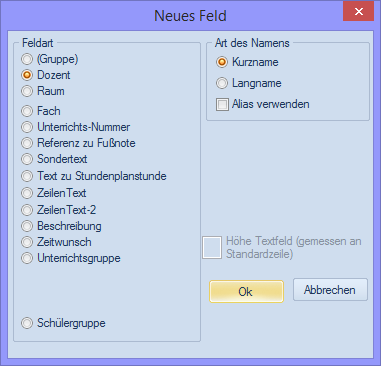
\includegraphics[width=.38\textwidth]{neues-feld}
	\vspace{-5pt}
	\caption{Neues Feld / Feld Ändern}
	\label{fig:neues-feld}
	\vspace{-25pt}
\end{wrapfigure}

Durch die Ansicht \texttt{Neues Feld} oder \texttt{Feld Ändern} können Sie neue Felder in der Darstellung bringen, oder ggf. die anzuzeigende Informationen eines vorhandenen Feldes ändern. Die Ansicht ist bis auf die beschriftung für beide Aktionen gleich.\\
\\
Im Bereich \texttt{Feldart} können Sie auswählen welches Attribut eines Unterrichts angezeigt werden sollte. Im \texttt{Art des Namens} hingegen, können Sie auswählen wie diese Informationen dargestellt werden soll. Attribute, die auf Ressourcen bezogen sind, haben hier typischerweise die Wahl zwischen der \texttt{Kurzname (Name)} und \texttt{Langname}. Bei Wert-orientiere Attribute, wie \texttt{Unterrichts-Nummer} oder \texttt{Sondertext} ist dieser Bereich leer.


\subsubsection{Tipps}

\begin{itemize}
	\item Die Nummerierung der Felder geschieht die Reihe nach. Falls bei einem Unterricht ein Feld nicht gepflegt würde kann es sein, dass die Informationen falsch ausgegeben werden. Daher, sollten sie Kopplungszeilen verwenden, möglichst alle Attribute ausfüllen. Sollten Sie das Attribut \texttt{Text} verwenden, ist es ratsam das \texttt{Text}-Attribut alle andere Unterrichte zumindest mit einem ``." \hspace{1pt} Zeichen zu belegen.
	\item Kopplungszeilen werden von Untis, sofern es die Darstellung betrifft, als eigenständige Unterrichte angesehen. Daher, sollten Sie Untis und nicht THM Organizer, für die Darstellung verwenden, kann es ratsam sein mehrere Dozenten oder Fächer als eigene Ressource, wie z.B. die Ressource ``Czermak/Runkel", zusammenzulegen. Dadurch kann man die Kopplungszeile vermeiden.
	\item Man kann bereits erstellte Felder in der Feinjustierungsbereich kopieren durch die Tastenkombination \texttt{STRG $+$ C} und einfügen durch die Tastenkombination \texttt{STRG $+$ V} dadurch ist man die neu Einstellung des Felds erspart, sollte man mehrere ähnliche Felder darstellen wollen.
	\item Felder der Feinjustierungsbereich können auch mit der \texttt{ENTF} Taste gelöscht werden.
	\item Mehrere Felder können gleichzeitig im Feinjustierungsbereich selektiert werden in dem man die \texttt{STRG}-Taste gedrückt hält und mehrere Elemente klickt. Dies kann hilfreich sein, wenn z.B. man mehrere Elemente verschieben möchte.
\end{itemize}



\section{Drück-Einstellungen}
\label{sec:druck-einstellungen}